% !TEX root = main.tex
\chapter{CÁC CÔNG NGHỆ VÀ CƠ SỞ LÝ THUYẾT}

\section{Xử lý ngôn ngữ tự nhiên}
\subsection{Vai trò của xử lý ngôn ngữ tự nhiên}
Xử lý ngôn ngữ tự nhiên (Natural Language Processing - NLP) là một lĩnh vực của trí tuệ nhân tạo (Artificial Intelligence - AI) tập trung vào việc phân tích và xử lý các bài toán liên quan tới ngôn ngữ tự nhiên giúp cho máy tính có thể hiểu, phân tích và khai thác thông tin từ chính các bài toán đó.

\begin{figure}[H]
    \centering
    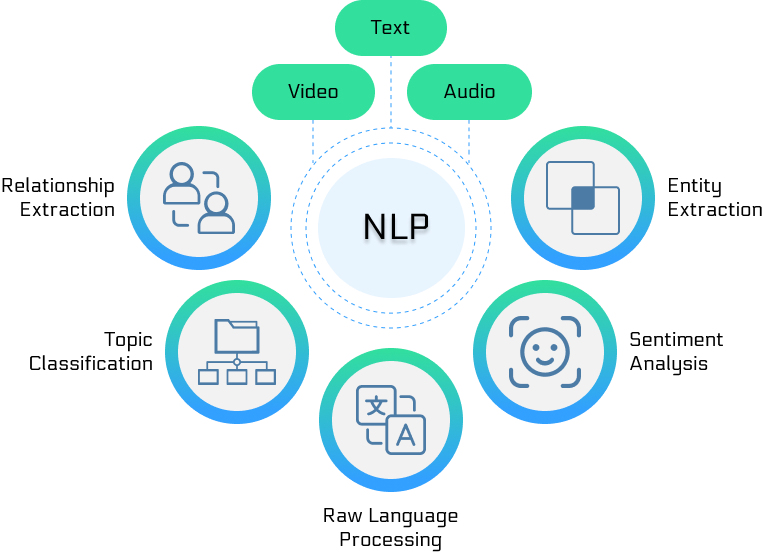
\includegraphics[width=0.8\textwidth]{images/chapter_02/img_01.png}
    \caption{Xử lý ngôn ngữ tự nhiên - Natural Language Processing}
    \label{fig:nlp}
\end{figure}

\noindent 
Khác với dữ liệu số hoặc dữ liệu có cấu trúc, dữ liệu văn bản ngôn ngữ tự nhiên có nhiều đặc điểm phức tạp, chẳn hạn như ngữ nghĩa, ngữ cảnh, cách sử dụng từ và cấu trúc câu. Do đó, NLP đóng vai trò quan trọng trong việc chuyển đổi văn bản thành dạng dữ liệu có thể đưa vào các mô hình học máy và học sâu xử lý.

\subsection{Biểu diễn văn bản và embedding}
Để cho máy tính có thể hiểu được văn bản, nội dung của văn bản đó sẽ được chuyển đổi sang dạng biểu diễn số. Một trong những phương pháp phổ biến để giải quyết được yêu cầu đó là chuyển đổi văn bản dưới dạng vector số, trong đó mỗi vector đều mang, chứa đựng các thông tin bao gồm: ý nghĩa, ngôn ngữ, cấu trúc của từ, cụm từ và câu. Các phương pháp truyền thống như Bag-of-Words hoặc TF-IDF chủ yếu biểu diễn vector dựa vào sự xuất hiện và tần suất của từ, vẫn chưa đủ khả năng
để phản ánh đầy đủ mối quan hệ ngữ nghĩa và ngữ cảnh của từ trong câu.

\vspace{\baselineskip}
\noindent
Embedding là một kĩ thuật chuyển đổi dữ liệu văn bản thô như từ ngữ, câu văn, hình ảnh hay là âm thanh sang một vector trong không gian đa chiều. Mỗi đơn vị mà có ý nghĩa tương đồng thì các vector của chúng sẽ được biểu diễn gần nhau trong không gian đa chiều đó. Nhờ vậy, embedding có thể giúp cho mô hình máy có thể hiểu và khai thác tốt hơn những đặc điểm ngữ nghĩa thay vì chỉ dựa trên sự xuất hiện riêng lẻ của từng từ.

\begin{figure}[H]
    \centering
    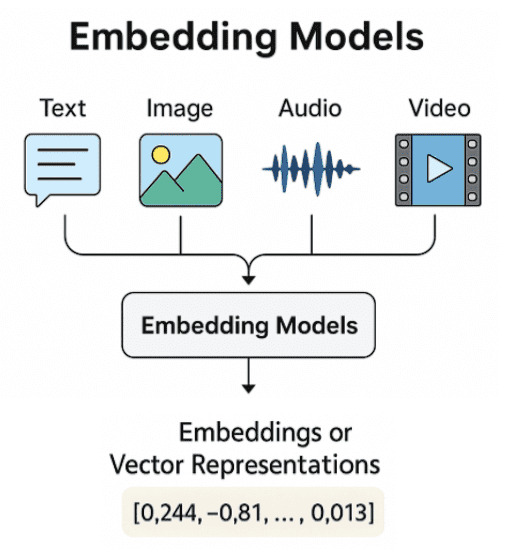
\includegraphics[width=0.4\textwidth]{images/chapter_02/img_02.jpg}
    \caption{Biểu diễn dữ liệu thô dưới dạng vector embedding}
    \label{fig:nlp}
\end{figure}

\noindent
Trong các hệ thống xử lý văn bản hiện tại, embedding là thành phần rất quan trọng trong việc hỗ trợ chuyển đổi dữ liệu dạng ngôn ngữ tự nhiên sang dữ liệu số, hay là vector để máy tính có thể hiểu, xử lý và tính toán được. Các vector embedding đó sẽ được đưa vào các mô hình học để thực hiện một số tác vụ như phân loại văn bản, tìm kiếm thông tin, phát hiện tương đồng và phân
tích ngữ nghĩa.

\vspace{\baselineskip}
\noindent
Đối với bài toán phân loại văn bản AI tạo ra, việc biểu diễn văn bản dưới dạng dữ liệu số có thể giúp cho các mô hình khai thác tốt đặc trưng từ dữ liệu đầu vào, tăng khả năng nhận diện được các văn bẳn do người viết hay do AI tạo ra. Tuy vậy, chất lượng biểu diễn các đặc trưng cũng góp phần cực kỳ quan trọng, ảnh hưởng trực tiếp đến kết quả đầu ra trong việc phân loại và đánh giá của mô hình.

\section{Mô hình Transformer và BERT}
\subsection{Kiến trúc Transformer}
Transformer là một kiến trúc mạng nơ-ron được thiết kế nhằm mục đích xử lý dữ liệu tuần tự, đặc biệt hiệu quả đối với các bài toán xử lý ngôn ngữ tự nhiên. Khác với các kiến trúc tuần tự như Recurrent Neural Network (RNN) và Long Short-Term Memory (LSTM), Transformer có khả năng xử lý các token trong chuỗi một cách đồng thời, không theo tuần tự. Có nghĩa là, mô hình sẽ tính toán mức độ liên quan của một token
so với các token khác tồn tại trong chuỗi. Nhờ đó, một token sẽ mang ý nghĩa phù hợp với ngữ cảnh, tức là phù hợp với ý nghĩa của câu đó mà không phải phụ thuộc vào mỗi bản thân của token đó.

\begin{figure}[H]
    \centering
    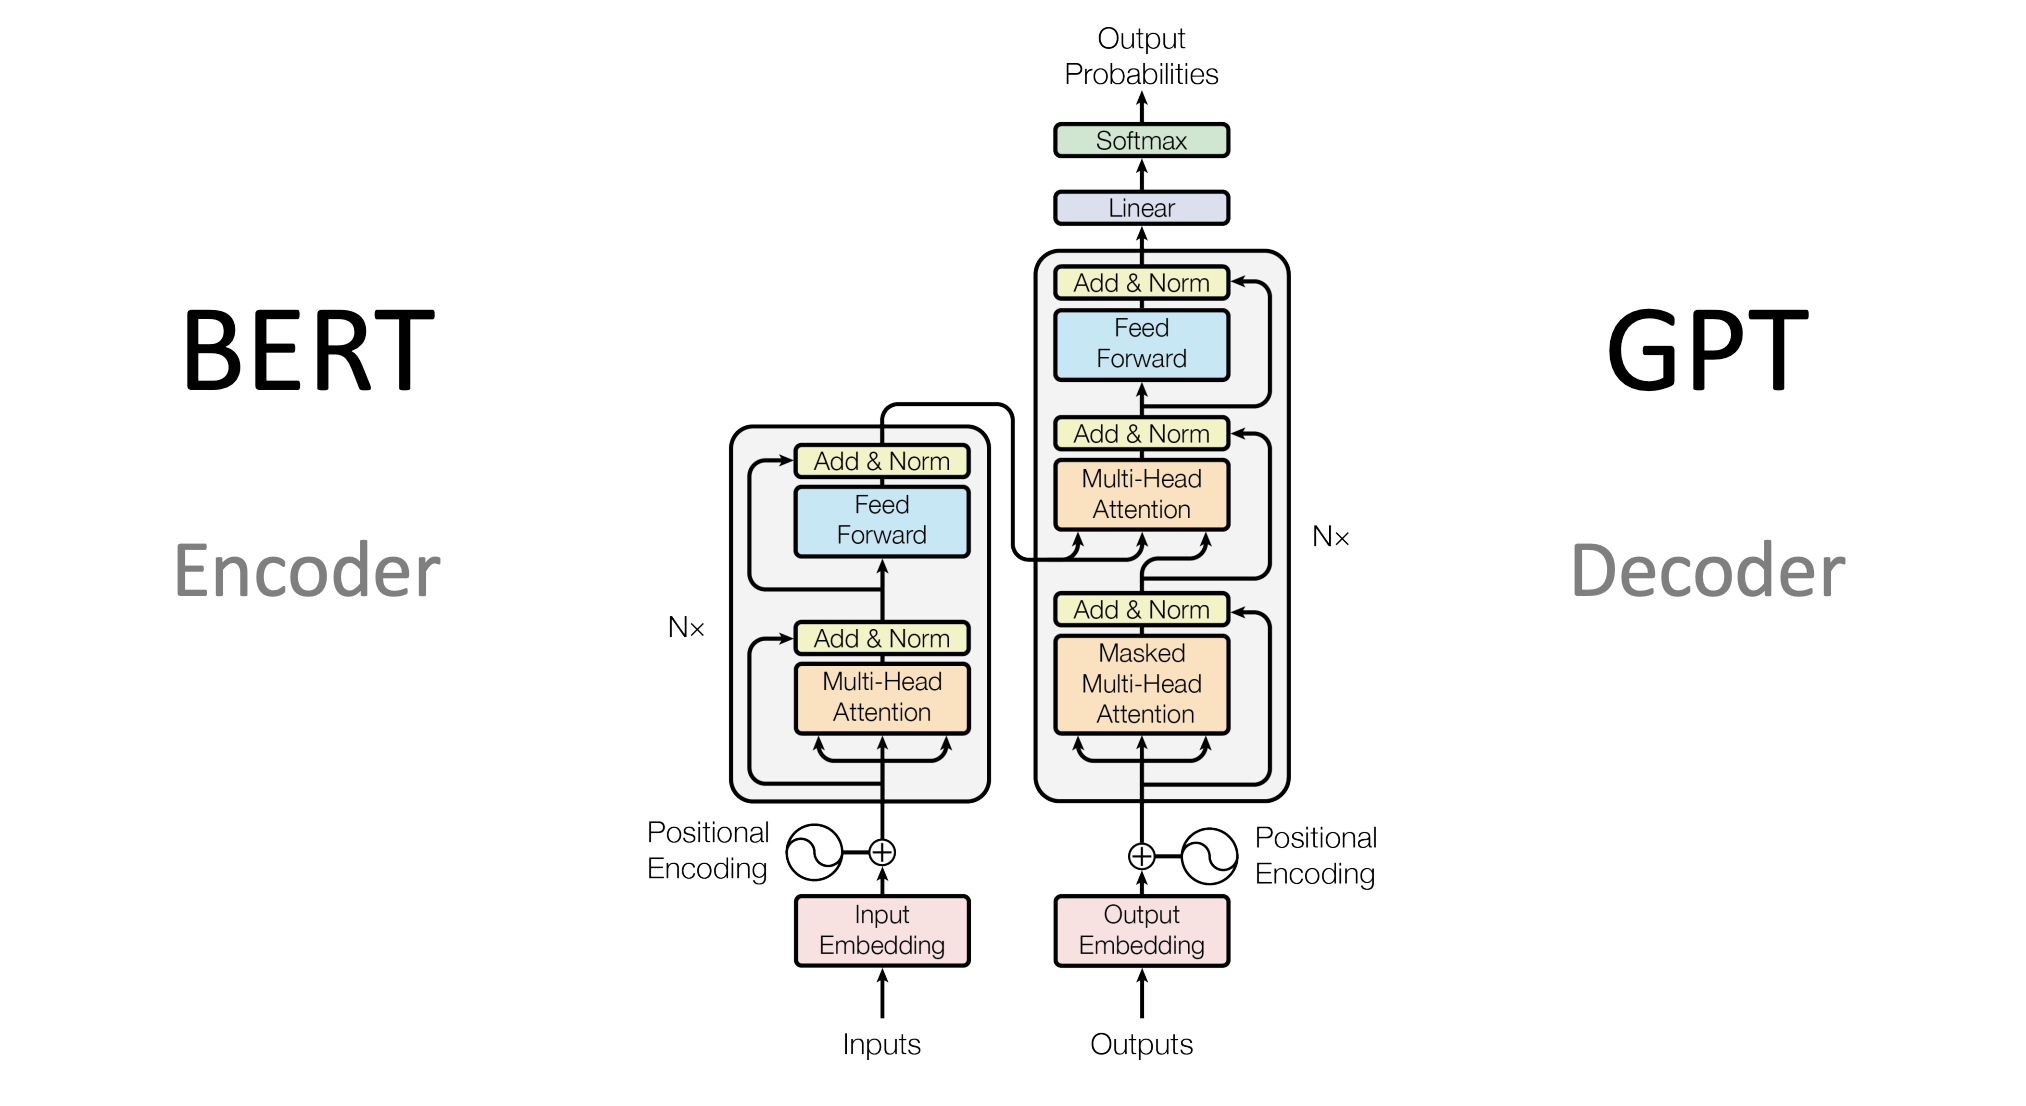
\includegraphics[width=1.0\textwidth]{images/chapter_02/img_03.png}
    \caption{Kiến trúc mô hình Transformer}
    \label{fig:nlp}
\end{figure}

\noindent
Cơ chế mà xác định mức độ quan trọng của từng token dựa vào các token lân cận có trong chuỗi được gọi là cơ chế tự chú ý (Self-Attention). Qua đó, Transformer có khả năng mô hình hóa các mối quan hệ phụ thuộc xa trong văn bản, tức là một token cần thêm thông tin từ một token rất xa trong văn bản, một đặc điểm quan trọng đối với các bài toán xử lý ngôn ngữ tự nhiên.

\vspace{\baselineskip}
\noindent
Transformer gồm tất cả là hai thành phần, Encoder và Decoder. Phần đầu là Encoder, dữ liệu đầu vào sẽ được chia thành các token (Tokenization) rồi sau đó sẽ embedding thành các vector. Tiếp theo, các vector đó sẽ được qua một lớp, gọi là Positional Embedding, lớp này sẽ có trách nhiệm embedding thành các vector có tính đại diện vị trí của từ trong chuỗi dữ liệu đó, ví dụ như: "I love AI" và "AI love I" thì mô hình nhìn có vẻ giống nhau nhưng thực tế
thì không phải vậy, thế nên là lớp Positional Embedding góp phần rất là quan trọng. Qua đó, ta sẽ có được một vector vừa có thông tin về ngữ nghĩa và vị trí của từ đó trong câu. Sau đó, các vector embedding sẽ được đưa vào lớp tự chú ý (Self-Attention) như đã nói ở trên, mỗi từ sẽ được ánh xạ thành ba thành phần: Query (Q) - từ này đang tìm kiếm cái gì, Key (K) - từ này yêu cầu cái gì, và Value (V) - thông tin thực sự mà từ này mang lại lại gì. Mỗi từ 
sẽ sử dụng Q để tính tích vô hướng so với các K của các từ còn lại, giá trị vừa tính được sẽ được chuẩn hóa thành các khoảng giá trị có thể xử lý được rồi sẽ đưa vào hàm Softmax để đưa thành các giá trị xác suất [0, 1].

\vspace{\baselineskip}
\noindent
Sau đó, dữ liệu sẽ đi qua lớp đa đầu tự chú ý (Multi-Head Self Attention), lớp này đảm bảo cho việc chú ý sẽ chạy song song, mỗi đầu tập trung vào một công việc riêng, ví dụ như một đầu tập trung vào mối quan hệ chủ ngữ - động từ, một đầu tập trung vào tính từ đó mô tả danh từ nào. Tiếp theo, dữ liệu sẽ được đưa vào lớp mạng nơ-ron truyển thằng (Feed-Forward Network), lớp này sẽ hỗ trợ cho việc đào sâu thông tin của từng từ hơn, ý nghĩa chính xác hơn và loại bỏ nhiễu kết hợp với các lớp
Add \& Norm để ổn định quá trình học hơn. Phần Decoder cũng có cấu trúc tương tự như Encoder nhưng thêm một lớp là Masked Multi-Head Attention, là lớp che đi các token phía sau của token đang xét để nó không biết trước thông tin. Điều này tránh rò rỉ thông tin trong quá trình học. Các khối Encoder và Decoder có thể lặp lại nhiều lần.

\subsection{BERT và BamiBERT}
BERT (Bidirectional Encoder Representations from Transformers) là một mô hình ngôn ngữ tiền huấn luyện được phát triển dựa trên kiến trúc Transformer Encoder. Nhờ vậy, mỗi token có thể khai thác thông tin từ hai chiều, phía trước và phía sau của token đang xét nên mô hình có khả năng nắm bắt tốt mối quan hệ các từ dựa trên ngữ cảnh của câu.

\vspace{\baselineskip}
\noindent
BERT được tiền huấn luyện trên một bộ lượng lớn văn bản thông qua nhiều nhiệm vụ học ngôn ngữ khác nhau, trong đó phổ biến nhất là mô hình ngôn ngữ che giấu (Masked Language Modeling - MLM). Cụ thể, trong nhiệm vụ này thì một số token trong câu sẽ bị che lại (masked) và mô hình có nhiệm vụ phải dự đoán các token bị che đó dựa vào các token còn lại. Quá trình này hỗ trợ cho mô hình BERT học được các đặc trưng của từ vựng, ngữ nghĩa và mối quan hệ giữa các thành phần trong văn bản.

\vspace{\baselineskip}
\noindent
Sau giai đoạn tiền huấn luyện, BERT có thể được fine-tune, tức là tinh chỉnh, huấn luyện trên tập dữ liệu của mình cho nhiều tác vụ khác nhau. Cụ thể trong bài toán phân loại văn bản, các biểu diễn thu được, tức là các vector embedding từ dữ liệu ban đầu từ BERT sẽ được đưa vào một lớp phân loại để dự đoán nhãn tương ứng. Cách tiếp cận này tận dụng kiến thức mà mô hình đã học được trong quá trình tiền huấn luyện thay vì xây dựng lại từ đầu

\vspace{\baselineskip}
\noindent
BamiBERT là một mô hình được xây dựng dựa trên kiến trúc BERT, được huấn luyện trên phần lớn các tập dữ liệu tiếng Việt với nhiều tác vụ khác nhau, bao gồm suy luận ngôn ngữ, nhận dạng thực thể, phân tích cảm xúc, phân loại chủ đề, phát hiện spam và phân tích khía cạnh.

\begin{figure}[H]
    \centering
    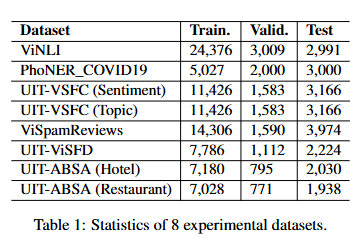
\includegraphics[width=0.6\textwidth]{images/chapter_02/img_04.png}
    \caption{Các tập dữ liệu dùng để huấn luyện BamiBERT}
    \label{fig:nlp}
\end{figure}

\noindent
Trong hệ thống, BamiBERT đóng vai trò là một mô hình biểu diễn các đặc trưng và sau đó biểu diễn này được sử dụng cho nhiệm vụ phân loại các lớp để đưa ra dự đoán. Việc sử dụng mô hình tiền huấn luyện giúp hệ thống tận dụng được các đặc trưng ngôn ngữ đã học trước đó và phù hợp hóa với bài toán phát hiện nội dung AI.

\begin{figure}[H]
    \centering
    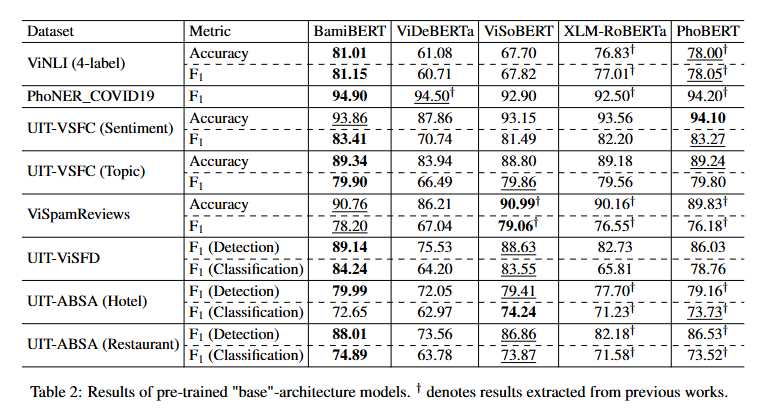
\includegraphics[width=1.0\textwidth]{images/chapter_02/img_05.png}
    \caption{Kết quả dự đoán của BamiBERT so với các mô hình BERT khác}
    \label{fig:nlp}
\end{figure}

\noindent
Lý do lựa chọn BamiBERT làm mô hình trích xuất, phân loại cho đồ án này là vì độ chính xác của mô hình tốt hơn hẳn so với các mô hình BERT trước dựa vào bảng kết quả (Hình 5). Tuy nhiên, có thể trong một số bài toán khác, hay cụ thể là bài toán phân loại văn bản AI này thì một số mô hình BERT khác có khả năng xử lý tốt và đưa
ra độ chính xác cao hơn. Do đó, bảng kết quả trên chỉ là thước đo cơ sở để lựa chọn mô hình BamiBERT nhưng về vấn đề xử lý hay độ chính xác cao hơn thì có thể các mô hình BERT khác tốt hơn so với BamiBERT.

\subsection{Token \texttt{[CLS]} và vector đại diện cho câu}
Trong kiến trúc BERT, token \texttt{[CLS]} (Classification) là một token đặc biệt được thêm vào vị trí đầu tiên của chuỗi đầu vào. Token này có nhiệm vụ tổng hợp toàn bộ thông tin của chuỗi đang xử lý thông qua các lớp Encoder của Transformer. Trong quá trình xử lý chuỗi, cơ chế Self-Attention sẽ cho phép token \texttt{[CLS]} tương tác với tất cả các token còn lại trong chuỗi, nhờ đó mà thu
được ngữ cảnh của toàn bộ văn bản trong chuỗi.

\begin{figure}[H]
    \centering
    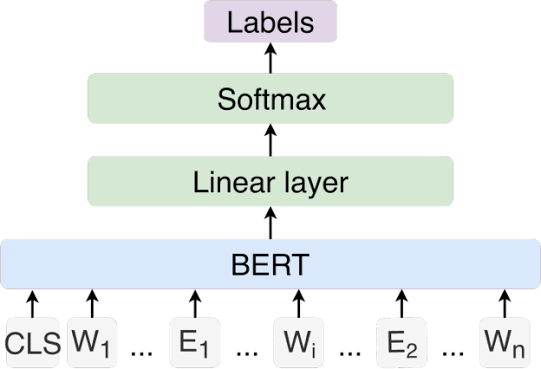
\includegraphics[width=0.6\textwidth]{images/chapter_02/img_06.png}
    \caption{Token \texttt{[CLS]} trong chuỗi}
    \label{fig:nlp}
\end{figure}

\noindent
Sau khi chuỗi đầu vào đi qua các lớp Encoder, mỗi token sẽ có một vector embedding tương ứng. Tuy nhiên, token \texttt{[CLS]} có một vector đặc biệt, là vector đại diện cho toàn bộ câu trong chuỗi. Vector này chứa toàn bộ thông tin ngữ cảnh của chuỗi đầu vào và được sử dụng cho các bài toán phân loại. Cụ thể, trong bài toán của đồ án này, vector biểu diễn của token \texttt{[CLS]} từ BamiBERT được sử dụng làm đầu vào cho Classification Head, sau đó vector này sẽ được
chuyển đổi thành các giá trị tương ứng cho hai lớp Human và AI cho bài toán, cụ thể các giá trị đó là giá trị logit.

\subsection{Classification head}
Classification head là một lớp của mô hình BERT, cho phép nhận đầu vào là vector đại diện của token \texttt{[CLS]} để thực hiện nhiệm vụ phân loại. Thành phần này là cầu nối giữa mô hình tiền huấn luyện và nhiệm vụ phân loại cụ thể.

\vspace{\baselineskip}
\noindent
Trong bài toán phân loại của đồ án, lớp classification head nhận đầu vào sẽ nhận vector đại diện của BamiBERT làm đầu vào. Sau đó, vector này sẽ được đưa qua một lớp gọi là lớp kết nối đầy đủ (Fully Connected Layer) để ánh xạ từ không gian nhiều chiều của BamiBERT sang không gian nhãn của bài toán phân loại của đồ án, tức là đồ án chỉ gồm có hai lớp, AI và Human nên không gian của bài toán này chỉ có
hai chiều và giá trị là logit. Tiếp theo, các giá trị này sẽ được trực tiếp đưa vào hàm Softmax để chuyển đổi thành các giá trị xác suất làm kết quả dự đoán.

\subsection{Fine-tune mô hình tiền huấn luyện}
Fine-tune là quá trình tiếp tục huấn luyện mô hình đã được tiền huấn luyện trên một tập dữ liệu cụ thể, một bài toán mà ta đang giải quyết. Tức là thay vì khởi tạo các tham số lại từ đầu thì quá trình này sẽ tận dụng các tham số mà mô hình này đã học được trong quá trình tiền huấn luyện, rồi điều chỉnh sao cho phù hợp với mục tiêu của bài toán.

\begin{figure}[H]
    \centering
    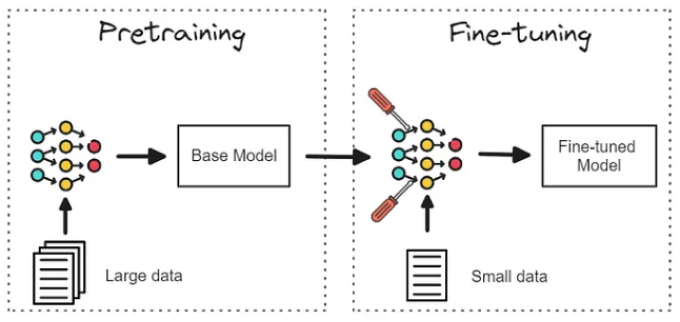
\includegraphics[width=0.8\textwidth]{images/chapter_02/img_07.jpg}
    \caption{Quá trình fine-tuning}
    \label{fig:nlp}
\end{figure}

\noindent
Đối với mô hình BamiBERT được sử dụng trong đồ án, giai đoạn tiền huấn luyện ban đầu đã phần lớn giúp cho mô hình đã học được các dữ liệu tiếng Việt. Tuy nhiên, mô hình này vẫn chưa được huấn luyện tối ưu cho bài toán phân loại, cụ thể là phân loại tin tức AI hay là Human. Do đó, đồ án thực
hiện fine-tune mô hình trên tập dữ liệu của bài toán, đồng thời kết hợp thêm lớp Classification Head để thực hiện phân loại văn bản đó là người hay AI tạo ra.


\section{Thuật toán diễn giải mô hình (Explainable AI - XAI)}
\subsection{Khái niệm Explainable AI}
Thuật toán diễn giải mô hình (Explainable AI) là một nhóm, tập hợp các phương pháp và kĩ thuật giúp cho con người cái cách mà một mô hình AI đưa ra dự đoán. Trong mô hình học sâu, thông thường thì quá trình dự đoán rất khó giải thích trực tiếp vì mô hình chứa rất nhiều tham số và thực hiện các thuật toán, quá trình 
tính toán cực kỳ phức tạp. XAI cung cấp phương pháp, thuật toán để giải thích mối quan hệ giữa dữ liệu đầu vào so với kết quả đầu ra của mô hình, điều này góp phần lớn cho việc giải thích minh bạch, dễ hiểu cho người dùng.

\begin{figure}[H]
    \centering
    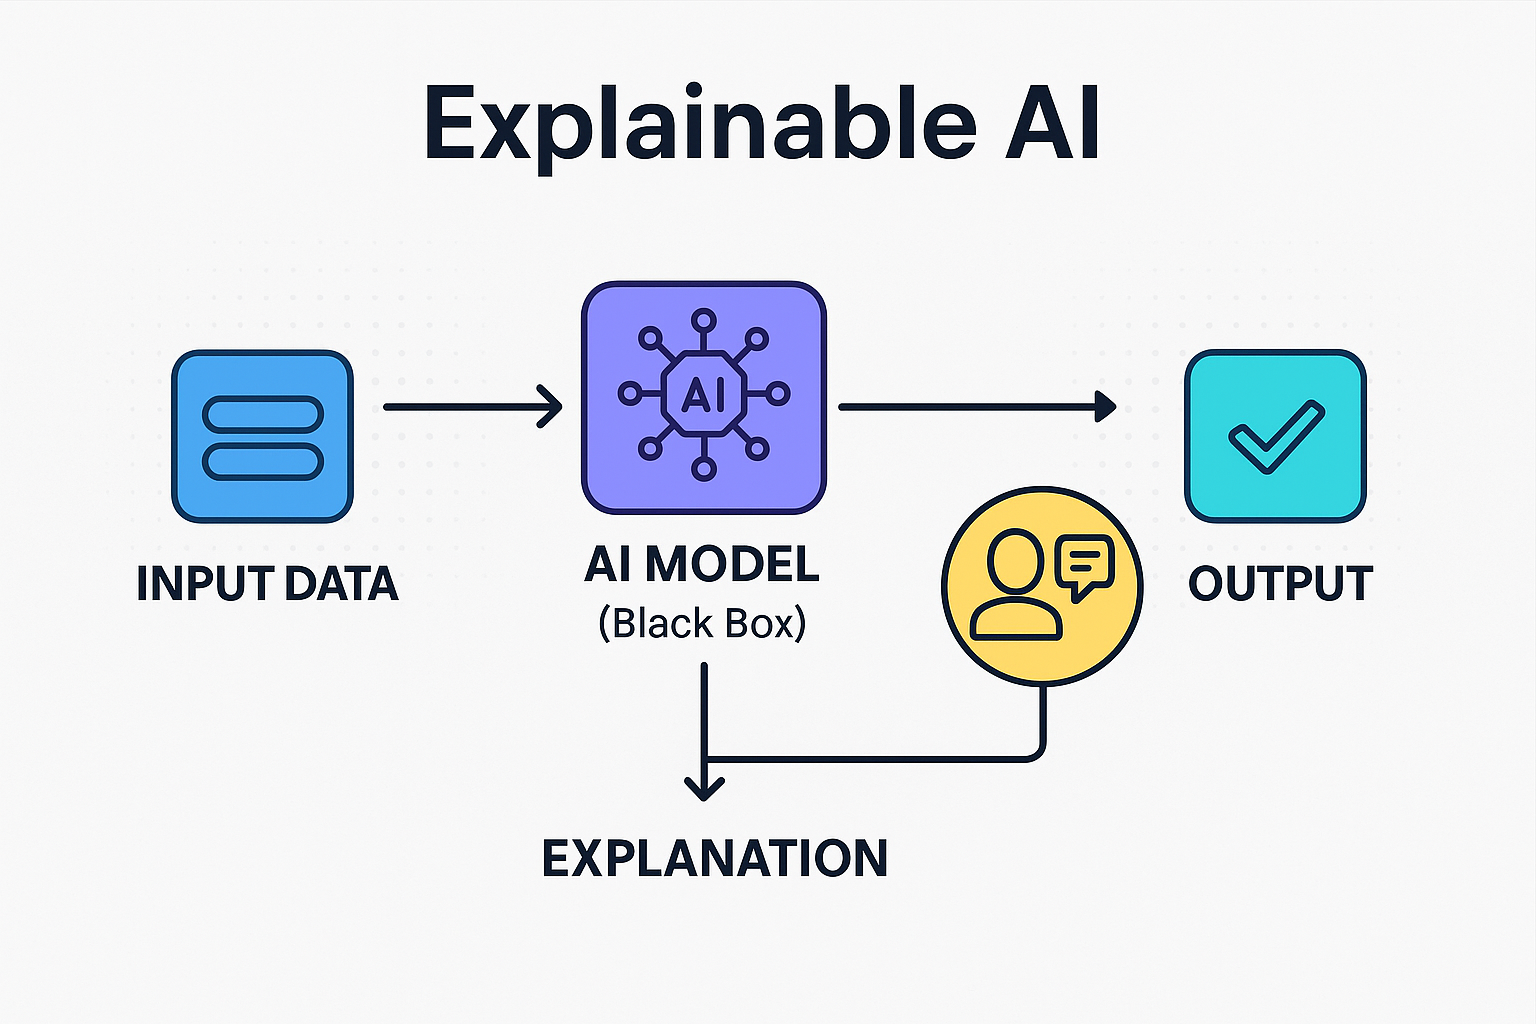
\includegraphics[width=0.6\textwidth]{images/chapter_02/img_08.png}
    \caption{Thuật toán diễn giải mô hình - Explainable AI}
    \label{fig:nlp}
\end{figure}

\noindent
Trong bài toán phân loại văn bản, thuật toán XAI được sử dụng để xác định những từ, token nào trực tiếp góp phần cho kết quả dự đoán, tức là mức độ ảnh hưởng của từ đó đối với kết quả mà mô hình dự đoán được. Ví dụ, trong đồ án này, khi mô hình dự đoán văn bản đó thuộc về lớp AI thì thuật toán sẽ trực tiếp xác định từ hay token nào trong văn bản đó
đóng góp đáng kể cho kết quả dự đoán. Nhờ vậy, kết quả của mô hình không những thể hiện dưới dạng nhãn dự đoán mà còn có thể cung cấp thông tin lý do vì sao lại đưa ra kết quả dự đoán đó. Nhờ đó, XAI hỗ trợ rất tốt trong việc phân tích lỗi và đánh giá các đặc trưng mô hình đã sử dụng trong quá trình phân loại.

\subsection{Thuật toán Integrated Gradients}
Thuật toán Integrated Gradients (IG) là một thuật toán XAI, sử dụng để xác định mức độ đóng góp của từng token so với kết quả dự đoán của mô hình. Phương pháp này sử dụng đạo hàm (gradient) của mô hình để phân tích mức độ ảnh hưởng của dữ liệu đầu vào đến đầu ra, tức là xem đầu ra của mô hình như thế nào khi thay đổi nhỏ đầu vào.

\vspace{\baselineskip}
\noindent
Ý tưởng chính của thuật toán này là xác định mức độ ảnh hưởng của từng đặc trưng dữ liệu đầu vào so với kết quả đầu ra của mô hình. Cách thức hoạt động của thuật toán như sau, đầu tiên IG sẽ bắt đầu từ đầu vào tham chiếu, tức là điểm xuất phát để thuật toán so với câu thực tế (baselines) và thay đổi dần cho đến dữ liệu thực tế. Tại mỗi bước, IG sẽ theo dõi sự thay đổi trong kết quả
dự đoán của mô hình khi dữ liệu đầu vào thay đổi một chút. Sau khi thực hiện qua tất cả các bước thì thuật toán này sẽ tổng hợp lại các kết quả để xem đặc trưng nào có ảnh hưởng ít nhiều so với kết quả dự đoán.

\setcounter{figure}{8}
\begin{figure}[H]
    \centering
    \[
    IG_i(x) = (x_i - x_i') \times \int_{\alpha=0}^{1} \frac{\partial F_i(x' + \alpha (x - x'))}{\partial x_i} \, d\alpha
    \]
    \caption{Công thức tích phân gradient tích hợp của thuật toán Integrated Gradients}
    \label{fig:integrated_gradients}
\end{figure}

\vspace{-0.3cm}
\noindent
Trong đó:
\begin{itemize}
    \item $x$: dữ liệu thực tế cần giải thích.
    \item $x'$: baseline.
    \item $F$: đầu ra của mô hình.
    \item $x_i$: đặc trưng thứ $i$.
    \item $IG_i(x)$: mức độ đóng góp của đặc trưng thứ $i$.
\end{itemize}

\noindent
Trong công thức trên, \(x_i - x_i'\) thể hiện sự khác biệt giữa đặc trưng thứ \(i\) của dữ liệu thực tế so với đặc trưng tương ứng của dữ liệu baseline mà ta đang xét. Ngoài ra, phần đạo hàm  \(\frac{\partial F_i}{\partial x_i}\) cho biết đầu ra của mô hình thay đổi như thế nào khi mà thuật toán thay đổi nhỏ đặc trưng thứ \(i\). Thay vì 
tính toán mức độ ảnh hưởng tại một thời điểm, thuật toán IG sẽ tính toán mức độ thay đổi này tại nhiều điểm trong quá trình đi từ baseline cho đến dữ liệu thực tế và tổng hợp các giá trị vừa tính được qua phép tích phân với $\alpha$ chạy từ 0 đến 1. Trong đó, 0 ở đây tức là vẫn đang ở baseline, 0.5 thì tức là đang ở giữa baseline và dữ liệu thực tế và 1 
đang ở ngay dữ liệu thực tế. Kết quả \(IG_i(x)\) cho biết mức độ đóng góp đặc trưng thứ \(i\) đối với kết quả dự đoán, giá trị càng lớn thì càng ảnh hưởng lớn đối với kết quả dự đoán. Nếu giá trị là dương, thì đặc trưng đang có xu hướng nghiêng ủng hộ phía lớp được dự đoán, còn giá trị âm thì ngược lại.

\vspace{\baselineskip}
\noindent
Ví dụ như trong đồ án phân loại văn bản AI này, các đặc trưng đầu vào đã được biểu diễn dưới dạng embedding của các token trong chuỗi văn bản. Do đó, thuật toán IG sẽ được sử dụng để xác định mức độ đóng góp của từng token đối với kết quả dự đoán của mô hình BamiBERT, những token có mức độ đóng góp lớn thì có ảnh hưởng lớn đến kết quả do mô hình BamiBERT dự đoán,
mức độ ảnh hưởng đó được tính thành một điểm được gọi là điểm đóng góp (Attribution Score).

\subsection{Attribution trong bài toán phân loại văn bản}
Attribution tức là mức độ đóng góp của các đặc trưng đầu vào đối với một kết quả cụ thể mà mô hình tạo ra. Cụ thể, đối với mô hình BamiBERT thì các đặc trưng này tương ứng với từng token trong chuỗi văn bản đang xét. Thông qua thuật toán IG, mỗi token sẽ được gán giá trị điểm đóng góp (Attribution Score) để biết được mức độ ảnh hưởng của token đó đối với kết quả dự đoán.

\vspace{\baselineskip}
\noindent
Trong bài toán phân loại văn bản AI, nếu attribution của một token có giá trị dương thì token đó có xu hướng hỗ trợ cho kết quả dự đoán của lớp đang xét, còn nếu token có giá trị âm thì ngược lại. Ngoài ra, độ lớn tuyệt đối của một token càng lớn thì token đó càng ảnh hưởng mạnh đến kết quả dự đoán của lớp mục tiêu. Nhờ vậy mà cái việc trực quan hóa khả năng diễn giải sẽ rất dễ 
hiểu cho người dùng.

\section{Mô hình ngôn ngữ lớn và ứng dụng trong hệ thống}
\subsection{Mô hình ngôn ngữ lớn (Large Language Model)}
Mô hình ngôn ngữ lớn (Large Language Model - LLM) là một loại mô hình AI được huấn luyện trên lượng lớn dữ liệu văn bản, có khả năng biểu diễn, đọc hiểu, xử lý và tạo ra văn bản bằng ngôn ngữ tự nhiên giống như con người, ví dụ như mô hình GPT, Gemini, Ollama,\dots Thông qua quá trình huấn luyện, mô hình LLM có khả năng nắm bắt, học được mối quan hệ giữa các từ, cấu trúc câu và ngữ cảnh,
từ đó có thể thực hiện nhiều tác vụ như là đọc và trả lời câu hỏi, dịch, tóm tắt văn bản hay là sinh nội dung.

\begin{figure}[H]
    \centering
    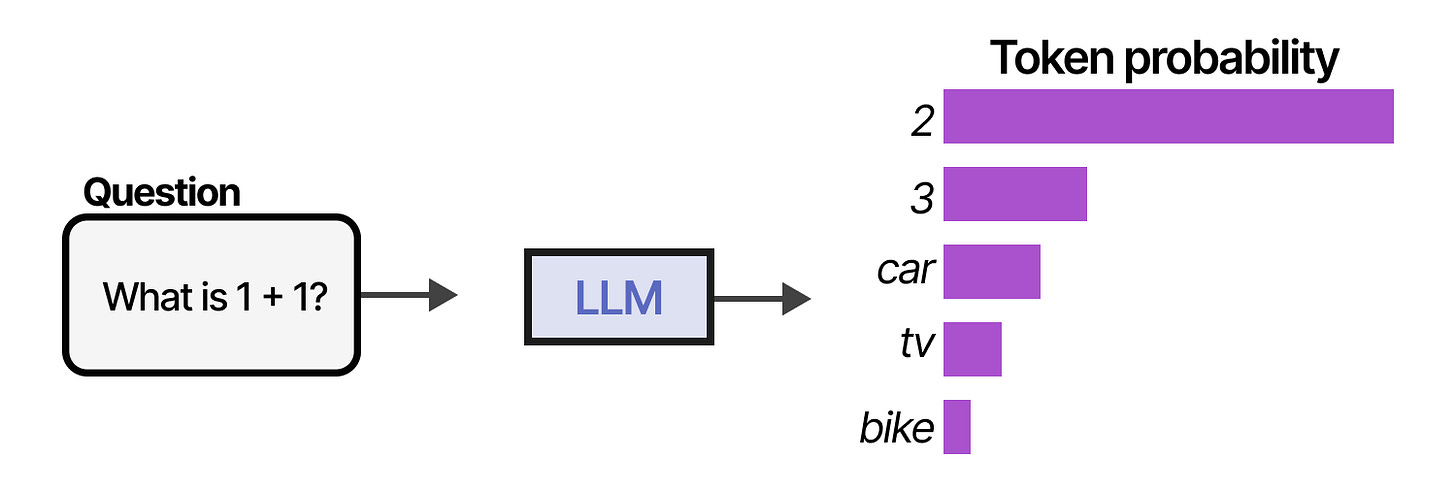
\includegraphics[width=0.8\textwidth]{images/chapter_02/img_10.jpg}
    \caption{Mô hình ngôn ngữ lớn - Large Language Model (LLM)}
    \label{fig:nlp}
\end{figure}

\noindent
Phần lớn các mô hình LLM đều hoạt động dựa trên kiến trúc Transformer, sử dụng cơ chế Self-Attention để khai thác tốt ngữ cảnh trong câu. Đối với quá trình sinh văn bản, LLM sẽ dự đoán token tiếp theo bằng cách tính xác suất của các token tiếp theo dựa trên các token hiện có và lựa chọn token dựa trên phân phối xác suất. Sau đó, token sẽ được thêm vào trong câu và quá trình này sẽ được lặp lại
cho tới khi câu được hoàn thiện. Ngoài ra, khác với các mô hình được xây dựng dựa trên một tác vụ cụ thể thì LLM có khả năng thực hiện nhiều nhiệm vụ khác nhau dựa yêu cầu do người dùng cung cấp dưới dạng prompt, nhờ đó mà mô hình có khả năng thực hiện nhiều nhiệm vụ khác nhau mà không cần phải huấn luyện lại mô hình từ đầu ứng với nhiệm vụ khác nhau.

\subsection{Ứng dụng LLM trong ứng dụng giải thích kết quả}
Trong các hệ thống AI hiện nay, thông thường các kết quả dự đoán của mô hình thường được biểu diễn dưới dạng nhãn, xác suất hoặc các giá trị định lượng thì sẽ gây khó hiểu cho người dùng trong việc hiểu nguyên nhân dẫn đến kết quả. Do đó, LLM thường được sử dụng bằng cách chuyển các giá trị định lượng đó sang giải thích bằng ngôn ngữ tự nhiên, nhờ vậy mà kết quả hệ thống sẽ trở nên minh bạch, dễ hiểu
hơn cho người dùng.

\begin{figure}[H]
    \centering
    
\includegraphics[width=0.5\textwidth]{images/chapter_02/img_11.jpg}
    \caption{Mô hình ngôn ngữ lớn (Gemini)}
    \label{fig:nlp}
\end{figure}

\noindent
Trong đồ án phân loại văn bản AI, IG được sử dụng để xác định mức độ ảnh hưởng, đóng góp của các token cho kết quả dự đoán của mô hình BamiBERT. Tuy nhiên, các giá trị số thường rất khó giải thích và khó hiểu cho người dùng. Do đó, trong đồ án này đã quyết định sử dụng mô hình Gemini để sử dụng và phân tích những giá trị định lượng đó, tạo ra những lời giải thích mà chỉ phụ thuộc vào các giá trị mà thuật toán, mô
hình đã tính ra bằng ngôn ngữ tự nhiên nhằm giúp cho người dùng hiểu được những thành phần nào trong văn bản có ảnh hưởng đến kết quả phân loại.